

\chapter{Computer Methods For Studying The Steady State Behaviour Of Theoretical}
\markboth{COMPUTER METHODS}{}

\section{Multi-Enzyme systems}

In this chapter a brief account will be given of computer methods which have been developed in order to facilitate the study by numerical solution of the otherwise intractable sets of simultaneous non-linear algebraic equations which define the stationary solutions of a multi-enzyme system.

In developing suitable methods two general aspects of such a study were considered particularly important. Firstly that the type of study which we have in mind is always experimental in nature, being in fact an experiment `in numero' on a theoretical system rather than, say, an experiment 'in vitro' on a reconstructed system, Because of this it is important that the computer methods used should allow the experimenter great flexibility in varying the values of parameters, in altering the actual structure of the system under consideration and in deciding what `measures' are to be made on the system. Ideally this flexibility will be achieved by having the experimenter `on line' to the computer and able to communicate with it in some sort of `biochemical language' which is simple to learn and use, and will allow him both to specify the metabolic system and to subsequently perform experiments on it. In practice any computer methods developed should be capable of evolving towards this ideal as `on-line' facilities become widely available.

The second aspect of importance is that the demands which such `in numero' experiments place on the available computer resources should not be so large that the user obtains only a poor response from the computing service, For our own purposes it was thought that the computer methods chosen should be able to perform a significant set of in numero experiments, say 100 S.S. and sensitivity matrix determinations on a medium sized system of 20 non linear enzymes, within a resource allocation which could be available to an average user on at least a daily basis.,
Keeping these requirements in mind the first decision is whether to employ an analogue or a digital computer.

\section{The Analogue computer}

For simulation work the analogue computer has two main advantages. Firstly that the analogue components, when suitably interconnected for a particular study, correspond directly to the `blocks' of the system being simulated and secondly that voltages on the components are directly representative of system variables. Secondly there is the ability to `interact' directly with the system by, for example, adjusting parameter(s) which correspond to potentiometer settings and then observing the response of system variables, often by direct oscilloscope display.

These advantages largely meet the requirement to be `onIine' and to have a simple means of carrying out, experiments on the system. However, the task of specifying the system in a form suitable to the analogue computer may still be formidable.

On the other hand the analogue computer has numerous disadvantages. Thus the size and non-linearity of, systems which can be simulated on any given computer is usually severely limited by the number of analogue components available and, furthermore, to avoid serious inaccuracy, system variables have to be `amplitude scaled' so that voltages lie within a limited range. Often repeated `rescaling' of a problem is necessary as an experiment is conducted. In addition there is always difficulty in repeating `runs' since analogue components are constantly developing minor faults.

For our own requirements the disadvantages just noted considerably outweigh the possible advantages, Thus ruling out the use of analogue computers for all but the smallest problems. For example, even with the quite large analogue computer available to us we would have been limited to the equivalent of about 7 nonlinear unimolecular enzymes with the further limitation that it would not have been easy to produce conveniently even an approximation to a sensitivity matrix.

\section{Digital computer systems}

By comparison the digital computer, if it is working at all, is highly accurate and completely reliable, usually being maintained by a service organisation. Furthermore there is, within reason, no limit to the size and non-linearity of the system being simulated except that the larger metabolic systems will require more time. In practice a further important advantage of digital machines is that, for mainly commercial reasons, far more effort is being devoted to * their development than is to that of analogue machines, so that each year they become more powerful and more widely available.

In recent years a large number of `simulation languages' have been written in which the general aim is to retain the undoubted advantages of the analogue computer whilst actually using a digital by machine, a useful review of some of these languages is by R.D. Brennan, (1964). In general these languages have been successful in allowing the user to work in terms of the `block' structure of his problem and in allowing him to easily load the structure and initialise the values of parameters. However, they have been less successful in allowing the user to `interact' with his system, since the proper development of such interaction must await the general availability of `conversational' operating systems at computing centres.

In order to discuss the particular methods which have here been used in devising a suitable 'simulation language' for the steady state properties of multi-enzyme systems. it will be necessary to give a brief description of certain concepts and terms commonly employed in digital computer science.

A computer system is indicated in the diagram below in which all details other than those required for a general understanding have been omitted

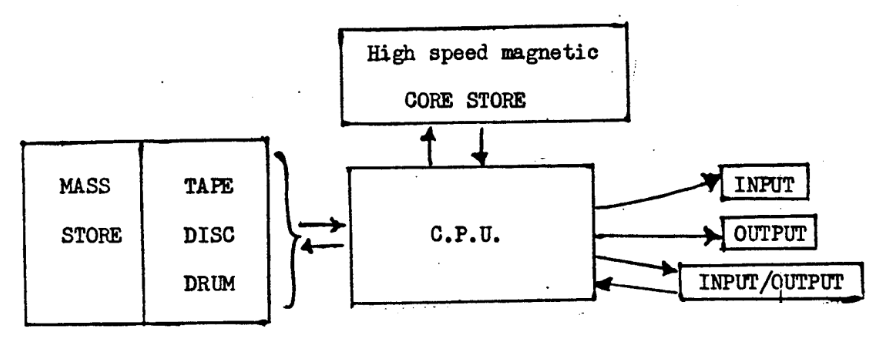
\includegraphics[max width=0.9\textwidth]{figure4_cpu}

The C.P.U. or `Central Processing Unit' is capable of reading binary stored patterns stored in locations within the high speed magnetic core store, and interpreting these patterns as 'instructions' which will control the next action of the C.P.U. When an instruction has been completed the C.P.U. will automatically fetch the next one from a designated location.

A modern machine will be capable of distinguishing and executing about one hundred distinct binary patterns as `legitimate' instructions each of which causes the C.P. U. to carry out a specific basic operation. These include `data transfer' instructions which move binary patterns, now considered as data, between registers in the C.P.U. and other registers, either in the core store or associated with various input, output, or mass storage devices. Input devices include teletypes, card and paper. punches, graph plotters, line printers and mass storage, includes magnetic tape, magnetic disc, magnetic drum etc. Other `data manipulation' instructions are concerned with carrying out operations on designated bit patterns, usually held in one or more registers belonging to the C.P.U, these include for example, arithmetic operations such as multiply and divide, logical operations such as `AND'ing two bit patterns etc. Usually the C.P.U. will fetch and execute instructions which lie sequentially in core, but certain instructions can determine from which core location the next instruction is to be fetched, so that, for example, it is possible to repeat a sequence of instructions until some condition is satisfied before continuing with further instructions.

A set of such instructions in core is called a `binary program' and, starting from a given instruction, will cause the C.P.U. to carry out a complete sequence of operations. For example it might read in a set of numbers, previously punched on paper tape and fed to a tape reader, store them as `data' in core, proceed to find their mean value and standard deviation and output the results on a line printer before returning to the start of the program ready to read in further input from the tape reader.

A modern computing system will provide a number of special. `system programs' which greatly simplify the task of the user and also help to ensure that the computer is being efficiently used.

One type of system program is an `operating system' or `O.S.' which has the important task of supervising the activities of all other programs (sequences of instruction in core, or on backing store) which are current. Thus if there are several programs in core at any one time a `multiprogramming' O.S. will allocate C.P.U. time to each in turn and will ensure that their input and output is connected with the appropriate peripherals. Or again the O.S. may maintain a `queue' of programs on a disc, so that the C.P.U. never runs out of work, and arrange for programs to be moved from and to backing store so that valuable core space is not wasted on inactive programs. An important goal for advanced O.S. is to allow a user to work from his own input/output station, just as if the computer were dedicated to him alone, this effect being achieved by the O.S `time sharing' the C.P.U. and other system resources amongst users active at any moment. This will eventually be important for simulation work (D. Garfinkel et al., 1970) since it will then be possible to `interact' with the system under study. Unfortunately such `conversational' O.S. have not proved easy to implement in any efficient way and are only now becoming available to the ordinary user in the U.K.

Another type of system program is a `compiler' which has the task of translating a program written in a `high level' source language into an equivalent binary program suitable for running on a particular machine. This relieves the user of the impossibly tedious task of breaking his problem down to the level of a series of binary coded machine instructions and instead allows him, to concentrate on describing his problem in one of the more or less readable high level languages. These include the well known `ALGOL' (ALGOrithmic Language) and `FORTRAN' (FORmula TRANslation) languages: compilers are available on most large machines to translate source programs, written in these languages into the equivalent binary code.

With the reasonably advanced O.S. presently available the user can call, by means of `control statements' which inform the O.S. of his wishes, any stored binary program such as a compiler and feed data to it from any specified input. This allows him for example to call further binary programs: which will receive as data the output of previous programs. If the O.S. provides conversational facilities he will in addition be able to interact with appropriately written programs. For example with a conversational 'editor program' or perhaps with his own suitably written simulation program.

\section{Design of suitable simulation system}

The actual implementation of a simulation system which broadly meets the requirements set forth at the beginning of this Chapter will depend very mach on the general facilities provided by the local computing centre. In our own case the situation was that the centre provided a reasonably advanced but non conversational 0.S. together with the `ALGOL' type of language compiler considered capable of producing nearly optimal binary code. With regard to `computing power' rough estimates indicated that the `KDF 9' computer, available at the time under this system, would, if carefully programmed, take about 10 minutes to complete the daily simulation work. Neither the limited basic computing power available to us nor the lack of a 'conversational' mode was thought likely to change appreciably for some years.

In these circumstances the basic decision was taken that the `structural input' for a simulation, that is the data which specifies the rate expression and how they are interconnected to give the functions, $\phi_{i}(S, P)$, would have to be converted by the available.

compiler into efficient binary code for evaluating the $\phi_{i}$. This was thought necessary because the `heart' of a simulation involves repeated numerical evaluation of the $\phi_{i}$ and any gain in efficiency at this level will immediately be reflected in the performance of the simulation program. A number of earlier simulation programs have not attempted to produce efficient code in this way and were correspondingly slow, thus limiting their usefulness. For example the earlier programs of Garfinkel were of this so called interpretative type (D. Garfinkel et al., 1970), which in effect meant that each evaluation of the $\phi_{1}$ involved the unnecessary work of rescanning a stored interconnection matrix, a step which in our method would be carried out only once at the compiling phase. G.H. BURGIN, (1966), who converted his originally interpretative `MIDAS' program so as to include a compilation phase claims an increase in `speed' of between 5 and 10 fold over the old version.

Since the `structural input' would not conveniently be in a form suitable for compilation it was decided to feed it as data to a program written by ourselves and designated the `precompiler'. The purpose of this `precompiler' was to convert the incoming structural data into a high level language and combine it with existing code to form a 'simulation program' suitable for passing on to the compiler. It was further decided that'this simulation program should, after compilation, be itself capable of receiving `commands' in a simulation language so that the user would not lose any of the advantages of purely interpretative simulation systems which usually provide a flexible means of controlling the actual simulation ``running phase''.

The use of a `precompiler' phase to construct and present for compilation a simulation program which can itself be driven by its own simulation language is shown in the figure opposite, and this general design has several results. Firstly it avoids the `inefficiency' disadvantages of a purely interpretative system since it ensures that basic and time consuming operations such as evaluation of the $\phi_{i}$, solution of differential equations and inversion of matrices will be in the form of nearly optimal binary code. Secondly it separates simulation into the two distinct phases of 'loading' and 'running' as indicated in the figure. This separation has the advantage that once a structure has been loaded it may be repeatedly investigated by supplying data, in the form of commands in the simulation language, to 2 stored binary version of the simulation program there being no need to return to the precompiler-compiler level unless it becomes necessary to alter the structure. Thirdly, it will be possible, depending on the sophistication of the precompiler and simulation program, for a user who is unfamiliar with programming to load his enzyme network using a notation which involves only simple algebraic and biochemical concepts and run his experiments by means of a series of simple `commands' interspersed with the necessary data. This will have the important effect of putting the power of the computing system directly into the hands of the investigator concerned. A further advantage in this respect is that although the main features of the simulation 'command' language are fixed it becomes a simple matter using the precompiler to add new commands as and when they are needed.

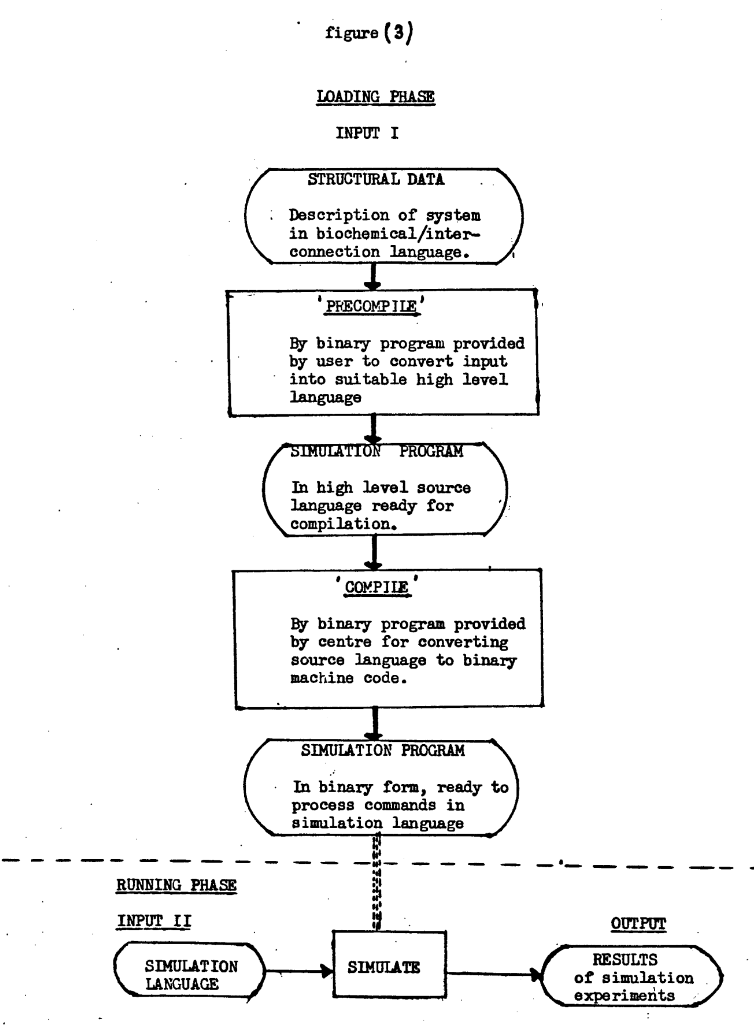
\includegraphics[max width=0.9\textwidth]{figure3_3.png}

Finally the production of the simulation program via a precompiler stage and its command language running technique are well suited for its efficient operation under conversational O.S. as they become available and little reprogramming will be necessary. In this respect the precompiler stage should result in a simulation program of high efficiency and with minimum demands on core storage Both of which are essential attributes if a reasonable response is to be obtained from the conversational 0.s. of the near future which will impose a heavy penalty on programs making large demands on time and core. The advantages of a `fast' simulation program are also very relevant to the `archive' problem. Thus the experiments to which we have referred consist in moving through `parameter-space' and observing the response of all system measures of interest. If the computation of the S.S. were very expensive in computer time it would become necessary to file or `archive' the results of experiments in case they were needed again for comparison with the results of later experiments as indeed they often would be. Such a strategy is, however, hardly practical on account of the difficulty of devising a filing system which could cope with the continuously expanding exploration of a virtually infinite parameter space, both from the point of view of classification and because of the sheer bulk of information. If, however, the computation of the S.S. is sufficiently fast no such problem need arise since it will be possible to recompute the same S.S. whenever it is required for purposes of comparison.

\section{Implementation on the KDF 9}

A simulation system of the general design just outlined was implemented on the Edinburgh University KDF 9 computer during 1968, several earlier versions having been discarded, and demonstrated at the FEBS summer school on `Computing Techniques in Biochemistry' in the same year. General impressions of my own and other, simulation programs are set forth by J.G. Reich, 1969.

In view of the impending removal of the KDF9 and also of proposed modifications to the high level language it was decided to keep the implementation as simple as possible within the general framework of having a `precompiler' and a 'simulation program'. With this in mind the 'biochemical language' was, for the meantime, taken as an algebraic specification of the rate-expression and of their use in forming the $\phi_{i}$ whilst the simulation language was restricted to being entirely numerical, with -ve numbers representing the various commands and +ve numbers the corresponding data. Both of these restrictions could of course be lifted in fuṭure versions of the simulation system, their purpose being merely to facilitate the first version. Thus the restricted biochemical language was suitable for direct compilation by the available compiler (Atlas Autocode). Whilst the precompiler, having no need to transform the incoming data, assumed more the form of an EDITOR which would edit the incoming text into the text of a previously filed simulation program. The editing aspects of the precompiler in fact proved so useful to myself and others that a `public' version, produced in collaboration with Dr. J.G. Burns of Edinburgh University, was made available to other users of the computing centre. A users guide to this is provided in the appendix.

\section{Editor (precompiler)}

This will not be described in detail since it is marginal to the enzyme simulation problem however its main features will be outlined since any future precompiler would almost certainly include them. The user operated the editor by means of issuing 'commands' which were followed, as appropriate, by the names of text files to be manipulated, line no's to be edited within the files and sections of text to be inserted. The basic operation of the editor was to take the text from a magnetic tape file, place it in core and edit it in accordance with the commands `DELETE', `INSERT' and `ALTER'. The resulting text could be passed to the compiler, by means of the command `RUN', for conversion into an equivalent binary program whilst the old version of the text on magnetic tape would automatically be overwritten by the new one unless the command `NOWRIT' was used. In addition text could be moved from one file to another by means of the command `BRANCH', inserted direct into a file from an input device by means of the command `FILE' or stored and retrieved from a `library' by means of special library commands. The editing system in its final form worked off one magnetic tape and maintained six text files each capable of holding a large program as well as a sizeable library.

In retrospect the editor turned out to be an essential part of the complete simulation system. Thus whilst enabling the non-programmer to 'load' the system using a standard sequence of editing instructions it also allowed the more sophisticated user to carry out the following operations.

i) Retain `on file' the text of all `networks' of interest. So that they could be modified when required, using the editor, and the new simulation program automatically established.

ii) Extend the simulation program itself by adding new routines and by developing special versions to study particular problems.

iii) Correct faults which from time to time were discovered in the simulation program.

It may be argued that the functions of the editor amounted to no more than `shuffling cards' or, as was the case at that time, editing paper tape. In practice, however, the ability to store, edit and list several large programs places the user in an altogether different position and makes feasible the type of activity which is essential to simulation. It turned out also that the programming techniques involved in writing the editor were very similar to those required for a simulation program capable of receiving a simple command language. In each case it is necessary to read in commands, look them up in a dictionary and then, using a `switch', select an appropriate sequence of routine calls which will carry out the command returning to read in the next command when execution is complete.

\section{The simulation language}

As mentioned earlier this was kept as simple as possible, being entirely numeric, both to reduce the size and complexity of the simulation program and also to keep the `commands' as concise as was possible. The integer part of each -ve number in the input stream will select a command and the first two decimal digits the particular `type' of that command if alternatives exist. A table of `commands' is shown opposite and an example of their use will be given in the next section. The main features of this table are as follows.

\subsection*{I. Selection of network}

If several networks have been previously loaded and the binary version of their corresponding simulation programs stored on magnetic tape it is possible to select among them using the command of type \kcmd{-0.XX}.

For example the command \kcmd{-0.02} means that the simulation program for a particular network which was previously compiled and filed in binary form in file number 2 is to receive any subsequent commands. If after some time it wished, say, to investigate the network held in file number 1 it is necessary for operations in file 2 to be brought to a close by means of the command \kcmd{-0.99} and the new system can be selected by means of the command \kcmd{-0.01}.

\begin{figure}
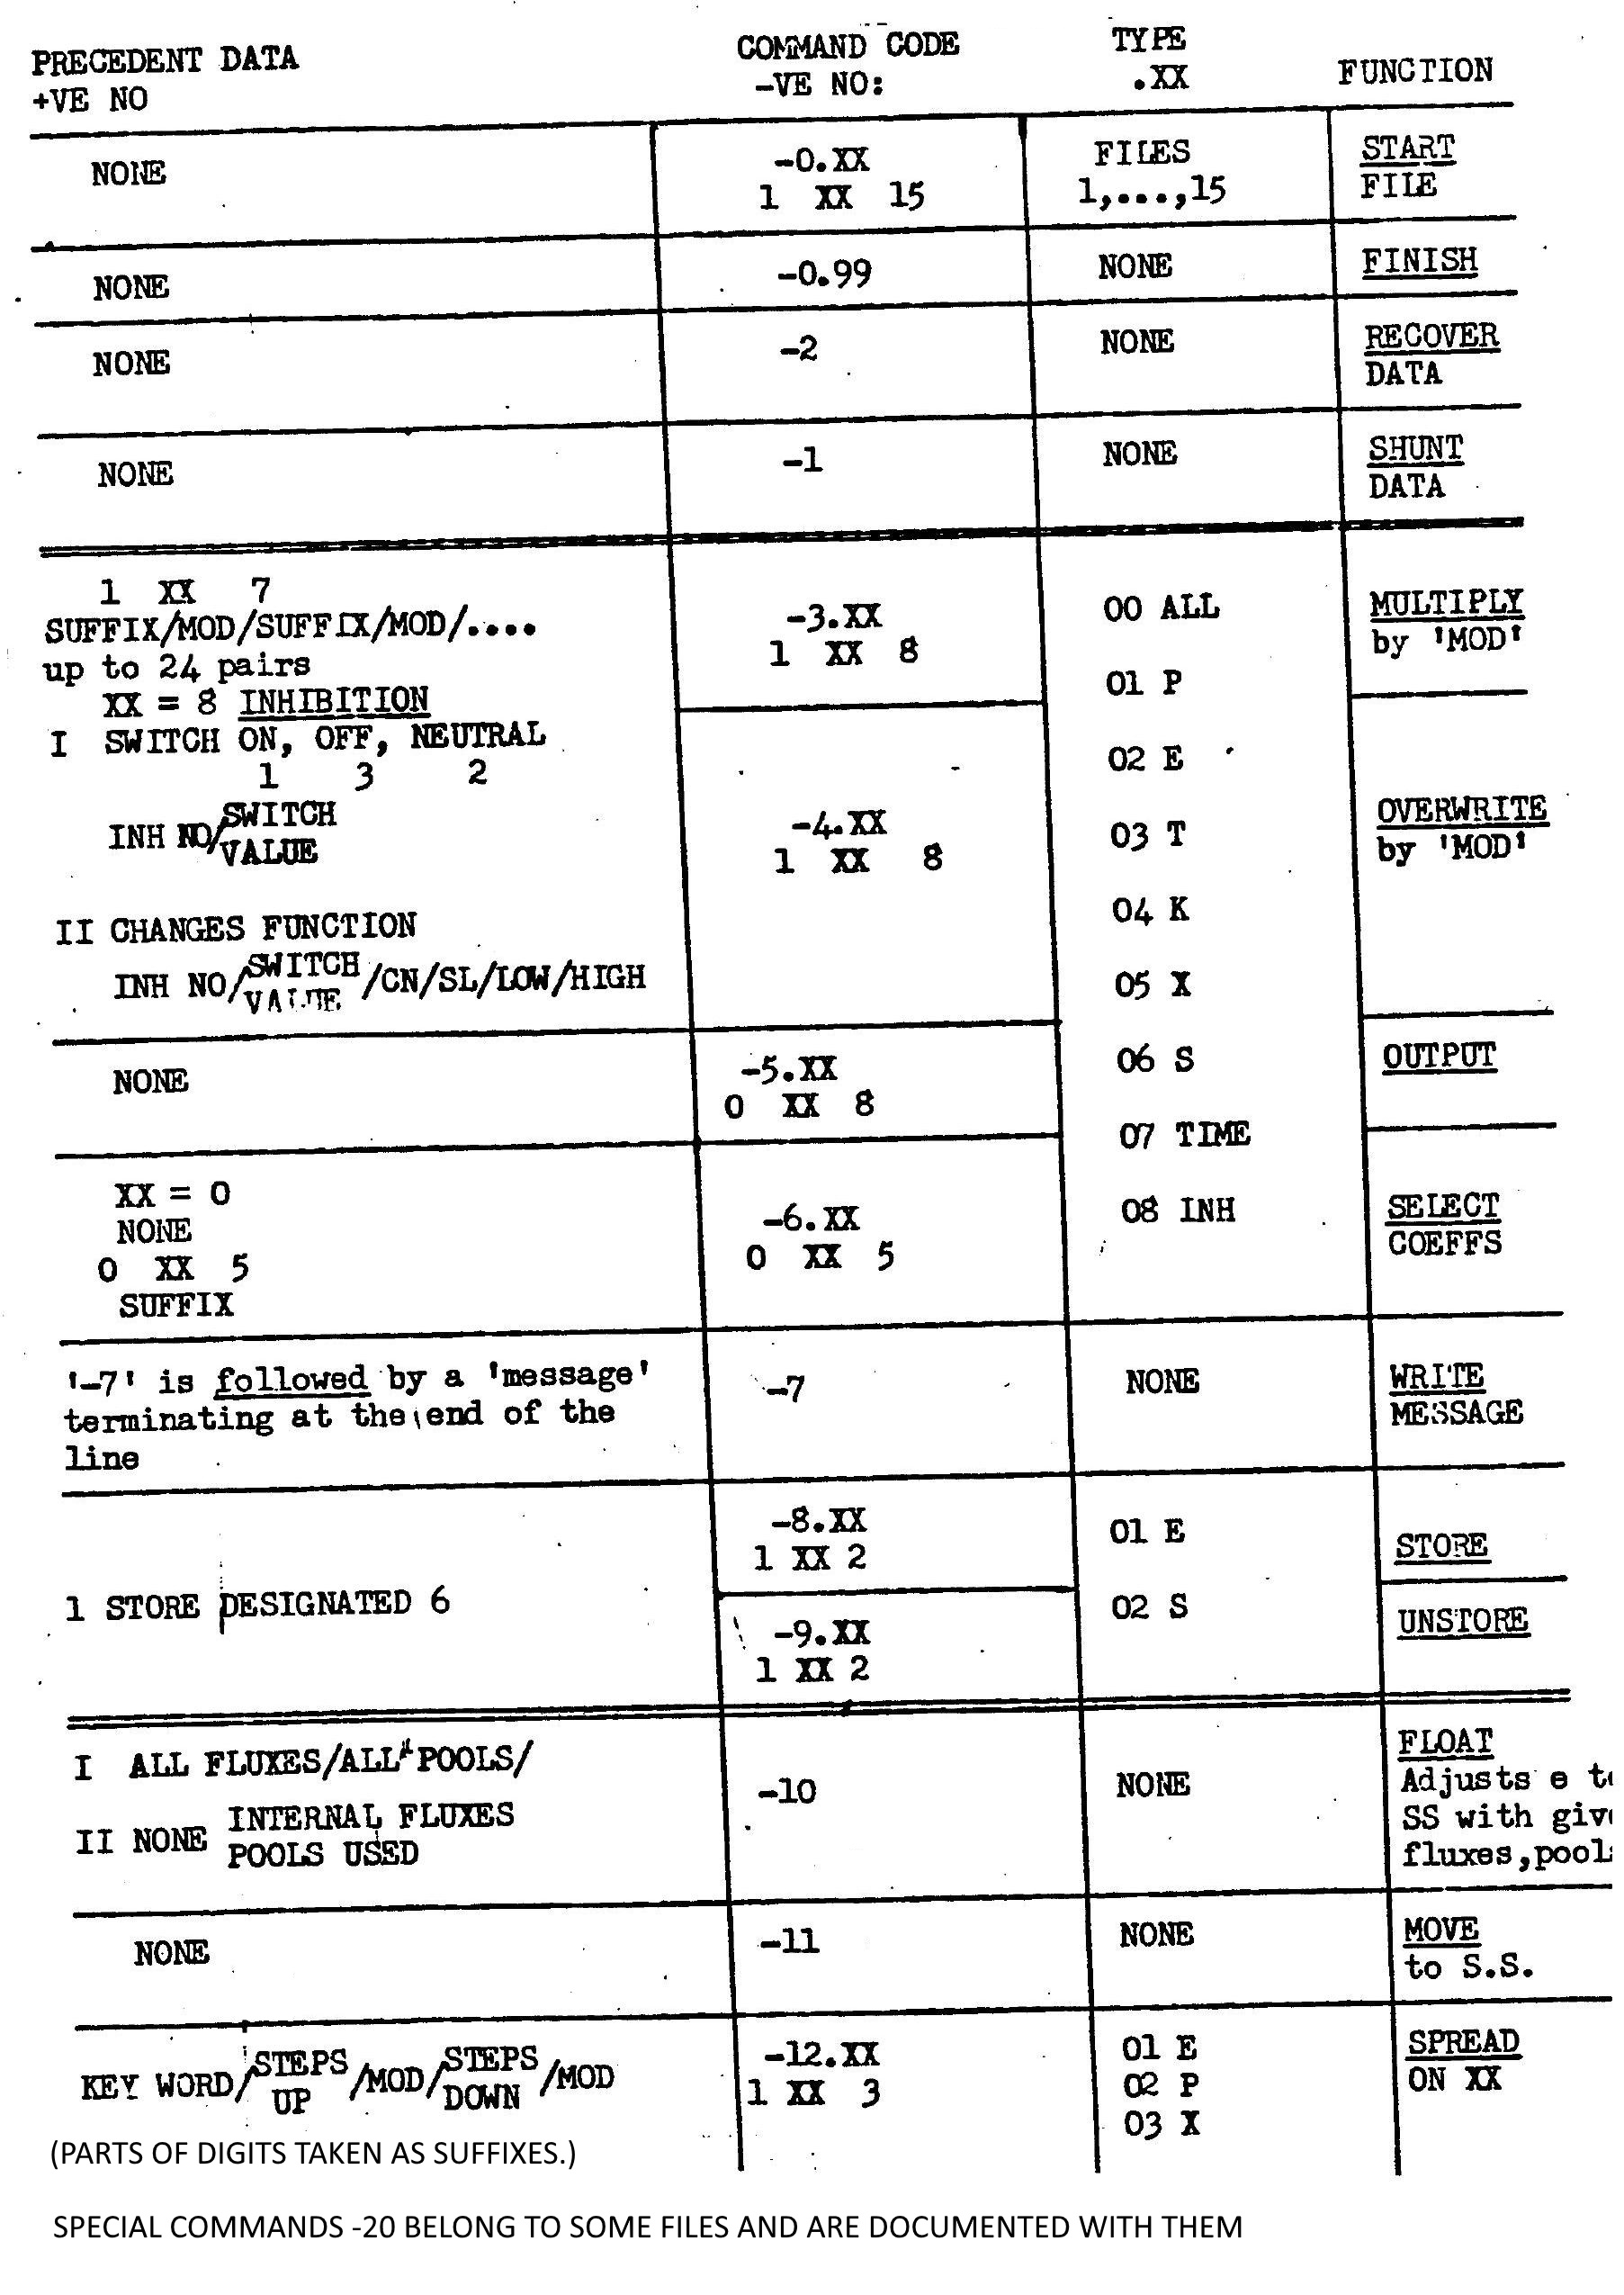
\includegraphics[max width=0.9\textwidth]{2023_01_30_a974a42f7b7381f3f940g-186}
\end{figure}

\subsection*{II. Parameter modification}

Parameters embedded within the expressions defining the $\phi_{i}$ can be altered in two ways, either by multiplying them by a specified factor or by replacing them with a new value.

Multiplication and replacement are brought about respectively by the commands \kcmd{-3.XX} and \kcmd{-4.XX} where \kcmd{.XX} specifies the particular type of parameter being modified as indicated in the table. For example the command \kcmd{-3.02} indicates that we wish to alter the quantity of an enzyme by multiplying its present quantity by some factor. Commands of this type must of course be accompanied by the appropriate `data' in the form of a set of +ve numbers preceding the command and provision is made for the user to provide as many pairs of numbers as required each pair specifying the enzyme to be changed and the amount by which it is to be multiplied respectively. For example the line

$11\qquad 10\qquad 4\qquad 5.2\qquad -4.02$

causes the operations $e_{1}=e_{1} \times 10 \mbox{ and } e_{4}=e_{4} \times 5.2$ to be carried out, where $e_{1}$ and $e_{4}$ represent enzyme quantities.

\subsection*{III. Output of the values of parameters and variables and printing of `messages'}

Output of values can be achieved by means of the command \kcmd{-5.XX} where the \kcmd{X} again selects the parameter or variable type which it is required to output. In this case the command always outputs the values of all members of a given parameter type and there is no need for precedent data. For example if there were 10 pools in a given system the command \kcmd{5.06} would cause the values of $S_{1}, S_{2}, \cdots S_{10}$ to be printed out, in that order. For convenience the command \kcmd{-5.00} causes a complete output, being equivalent to \kcmd{-5.01}, \kcmd{-5.02} $\ldots$ \kcmd{-5.08}. In order to improve the legibility of the output the command \kcmd{-7} can be \underline{followed} by any `message', the effect being cancelled when the end of the line is reached.

\subsection*{IV. Selection of sensitivity coefficients for subsequent output.}

Commands of the type {\tt \textquotesingle -6.XX'} will select which parameters the coefficients are to be found with respect to. Thus whenever a S.S. is subsequently computed only selected rows of the generalised sensitivity matrix $\left[C_{P_j}^{S_{i}, F_j, M_{K}}\right]$ will be outputted. In this case, the \kcmd{.XX} specifies the type of parameter, $P, X$, etc, and a list of the +ve numbers preceding the command specifies which members of the type vector, $X_{1}, X_{2}$ etc, are required. For example the two command lines,

$\begin{array}{llll}1 & 5 & 7 & -6.01 \\ 4 & & &-6.05\end{array}$

will select for subsequent output the rows with respect to $P_{1}, P_{5}, P_{7}$ and $X_{4}$ respectively. The command {\tt -6.00} will select \underline{all} rows of type $C_{\alpha i} $ i.e. the block coefficients, and requires no precedent data.

\subsection*{V. Storage and Retrieval of Values}

Often it is convenient, after a sequence of parameter variations for example, to, return to an earlier set of parameter and variable values. There are several commands which are of use in this situation. Thus \kcmd{-1} will `shunt' the existing values of all parameters, variables, matrix elements etc. onto magnetic tape and \kcmd{-2} will `recover' them. The commands \kcmd{-8.XX} and \kcmd{-9.XX} perform a similar function but are more limited, the \kcmd{.XX} referring to manipulation of either the pool or the enzyme quantity vectors by themselves. For example the command \kcmd{-8.01} will store the existing enzyme values and the command \kcmd{-9.01} issued subsequently will then overwrite any new enzyme vector which may have arisen with the original one which was stored.

\subsection*{VI. Computation and output of S.S.}

A number of commands are concerned with causing S.S. calculations to be performed and also with outputting the results. Thus \kcmd{-1}, which can be called after any parameter adjustments, will cause variables to move to their S.S. values and will automatically output all pools, fluxes, special measures and any coefficients which have been selected.

If it is required to compute and output a sequence of S.S.solutions corresponding to a steadily increasing value of some parameter this can be achieved concisely by means of the `SPREAD' command of type \kcmd{-12.XX}. For example the line

{\tt \textquotesingle 1010203 \qquad  3 \qquad 2 \qquad 3 \qquad -12.03\textquotesingle}

will cause $\mathrm{X}_{3}, \mathrm{X}_{2}$ and $\mathrm{X}_{1}$ specified in the leading `KEYWORD', each to be modulated up and down by three powers of 2, thus computing 9 S.S. around the original position.

\subsection*{VII. Adjustment of enzymes to achieve a given S.S.}

A further useful command is \kcmd{-10} or `FLOAT' which, when supplied with precedent data for all pools and `independent fluxes' will adjust or `float' the values of the enzymes carrying 'dependent' fluxes so that a perfect steady state is achieved corresponding to these specified pools and independent fluxes. Since one may often wish to model a situation where relative fluxes and pools are roughly known this command has proved useful.

\section{Loading and running a system}

To make clear the steps which are involved in using the simulation system we will consider the six enzyme divided pathway network shown below:

\begin{center}
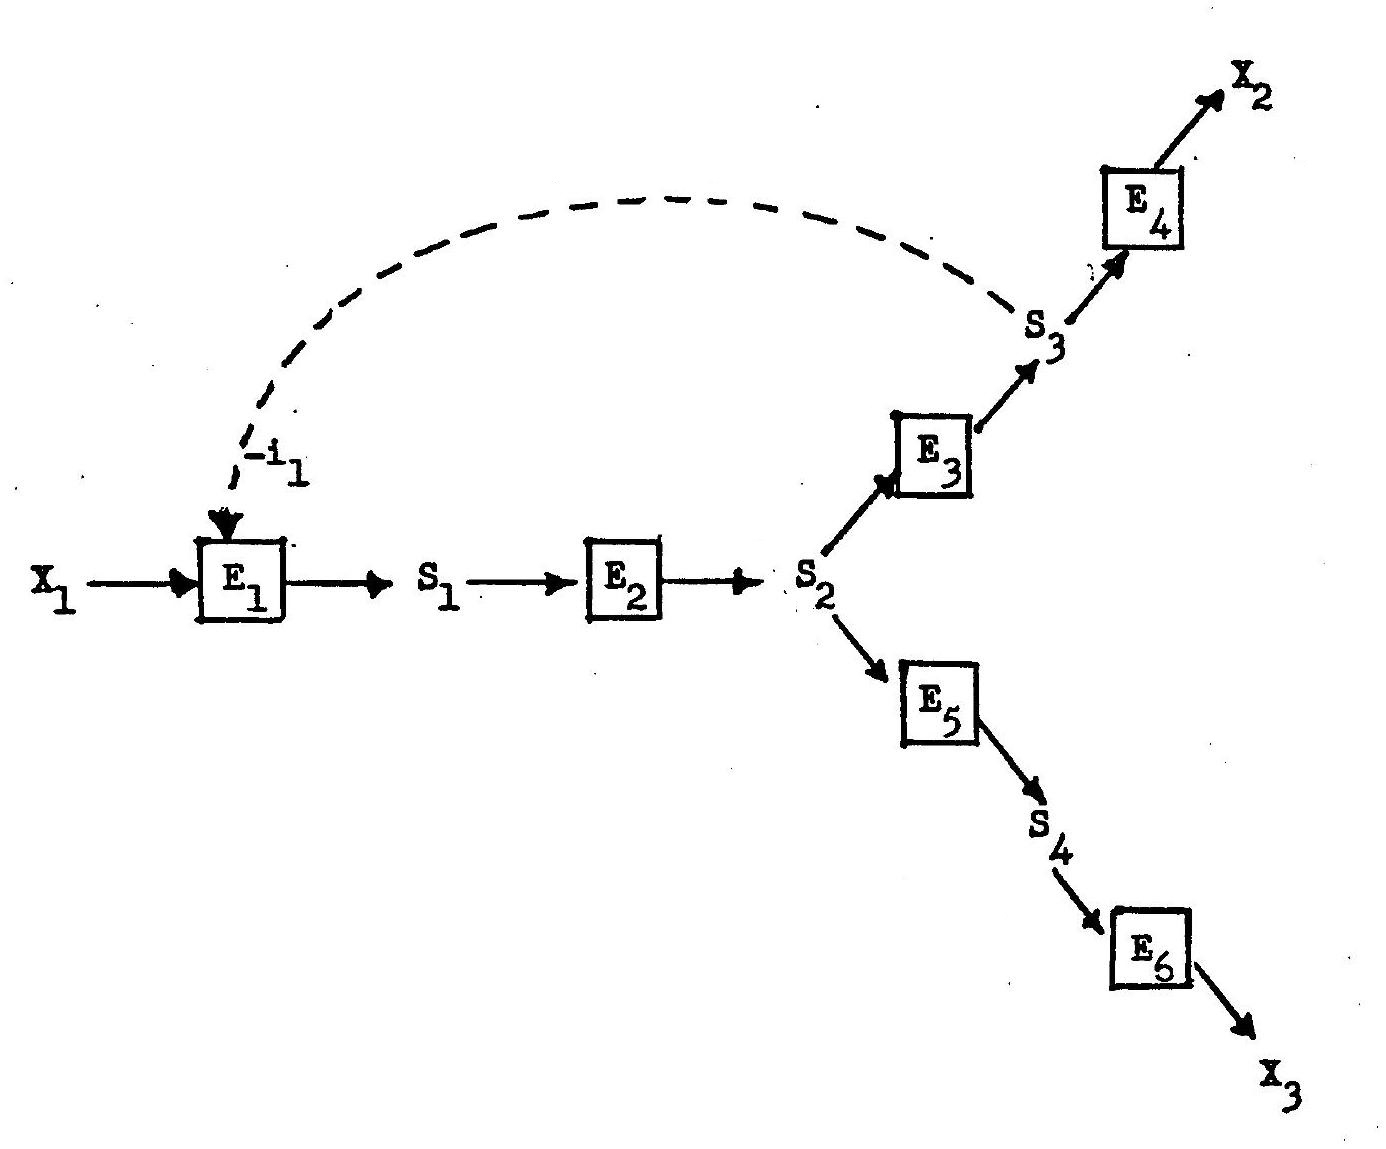
\includegraphics[max width=0.75\textwidth]{2023_01_30_a974a42f7b7381f3f940g-191}
\end{center}

The network involves a metabolic inhibition $i_1$, and as an example, is supposed to be a subsystem in an expanding space which has an exponential growth constant $P_{1}$

\section{Loading}

Below are set out the main stages involved in loading the system via the precompiler. The notation used is similar, but not identical, to that actually used on the computer, and corresponds to the notation of CM.I and II. The input is typed onto paper tape or cards or, if an on-line system is available, perhaps direct into the computer. The precompiler stage can detect certain `obvious' errors in the input and `abort' the loading phase, if these are sufficiently severe.

\section{Details of step}

{\renewcommand{\arraystretch}{2}
\begin{tabular}{lp{10cm}}
STEP & DETAILS OF STEP \\ \\
A & Provide correct control. statements to activate the EDITOR/
precompiler and find the relevant text for the required
simulation program from among the editors files. \\
%
B &
Type out the six flux expressions giving the flux at each of the six blocks in terms of the surrounding pools etc. Thus

$F_{1}=E_{1} t_{1}\left(X_{1}-S_{1} / K_{1}\right) \times i\left(1, S_{3}\right)$

$ F_{2} = E_{2} t_{2}\left(S_{1}- S_{2} / K_{2}\right) / \left(1 + S_{1} / P_{2}+ S_{2} / P_{3}\right)$

etc \\
%
C &
Show how the 'Fs' combine to produce the pool rates of change, including the effects of expansion. Thus

$\phi_{1}=F_{1}-F_{2}-P_{1} S_{1}$

$\phi_{2}=F_{2}-F_{3}-P_{1} S_{2}$

etc \\
D &
Taking the two independent fluxes as the outputs $F_{4} F_{6}$ show how the dependant fluxes are related to them

$\mathrm{F}_{3}=\mathrm{F}_{4}+\mathrm{P}_{1} \mathrm{S}_{3}$

$\mathrm{F}_{5}=\mathrm{F}_{6}+\mathrm{P}_{1} \mathrm{S}_{4}$

$F_{2}=F_{3}+F_{5}+P_{1} S_{2}$

etc \\
%
E &
Write down expressions defining any special `measures'
which are currently of interest. For example the ratio
of fluxes in the two pathways
%
$$ M_{1}=\frac{F^{4}}{F_{6}} $$ \\
%
F &
Assign values to all parameters and I.C. to pool
variables any not assigned will automatically have
value unity. Indicate which binary file should hold
the compiled version of the simulation program

$ \mathrm{P}_{1}=0.001 $

$ \mathrm{P}_{2}=10 $ \\
%
G &
Provide a title for the network, which will be automatically printed out whenever it is run. Thus
`SIX ENZYME DIVIDED RATHWAY WITH INHIBITION' \\
%
H &
Provide, in high level programming language, the code necessary to execute any special commands which you wish to add to the basic simulation language for this investigation, these to be numbered from 20 upwards. Thus

$ 20: \ldots\ldots $

$ 21: \ldots\ldots $
\end{tabular}}

In principle sections $C$ and $D$ could be omitted since they duplicate information already contained with the rate expressions of B.

However they do not represent a large amount of input and they have been included rather than employing a more complex form of precompiler. The representation of inhibition is simplified by means of a standard inhibition routine $i(S, n)$ available within the standard simulation program. Any number of functions can be set up in this way, each being defined by four parameters which control its' slope, maximum inhibition, etc. and which can themselves be modified via the simulation language.

When all sections have been loaded the precompiler incorporates them into the text of the standard simulation program held in its files and feeds the resulting complete program to the compiler. If the program compiles successfully, that is has no obvious errors in it, the resulting binary version will be placed into the designated binary file where it can be repeatedly accessed for use in the 'run' phase by the appropriate {\tt -0.XX} command.

\section{Running}

The system just loaded can now be accessed for experimentation indefinitely unless it is required to alter its structure or perhaps add some extra 'commands'. The following sequence of commands exemplifies one such experiment.

\begin{center}
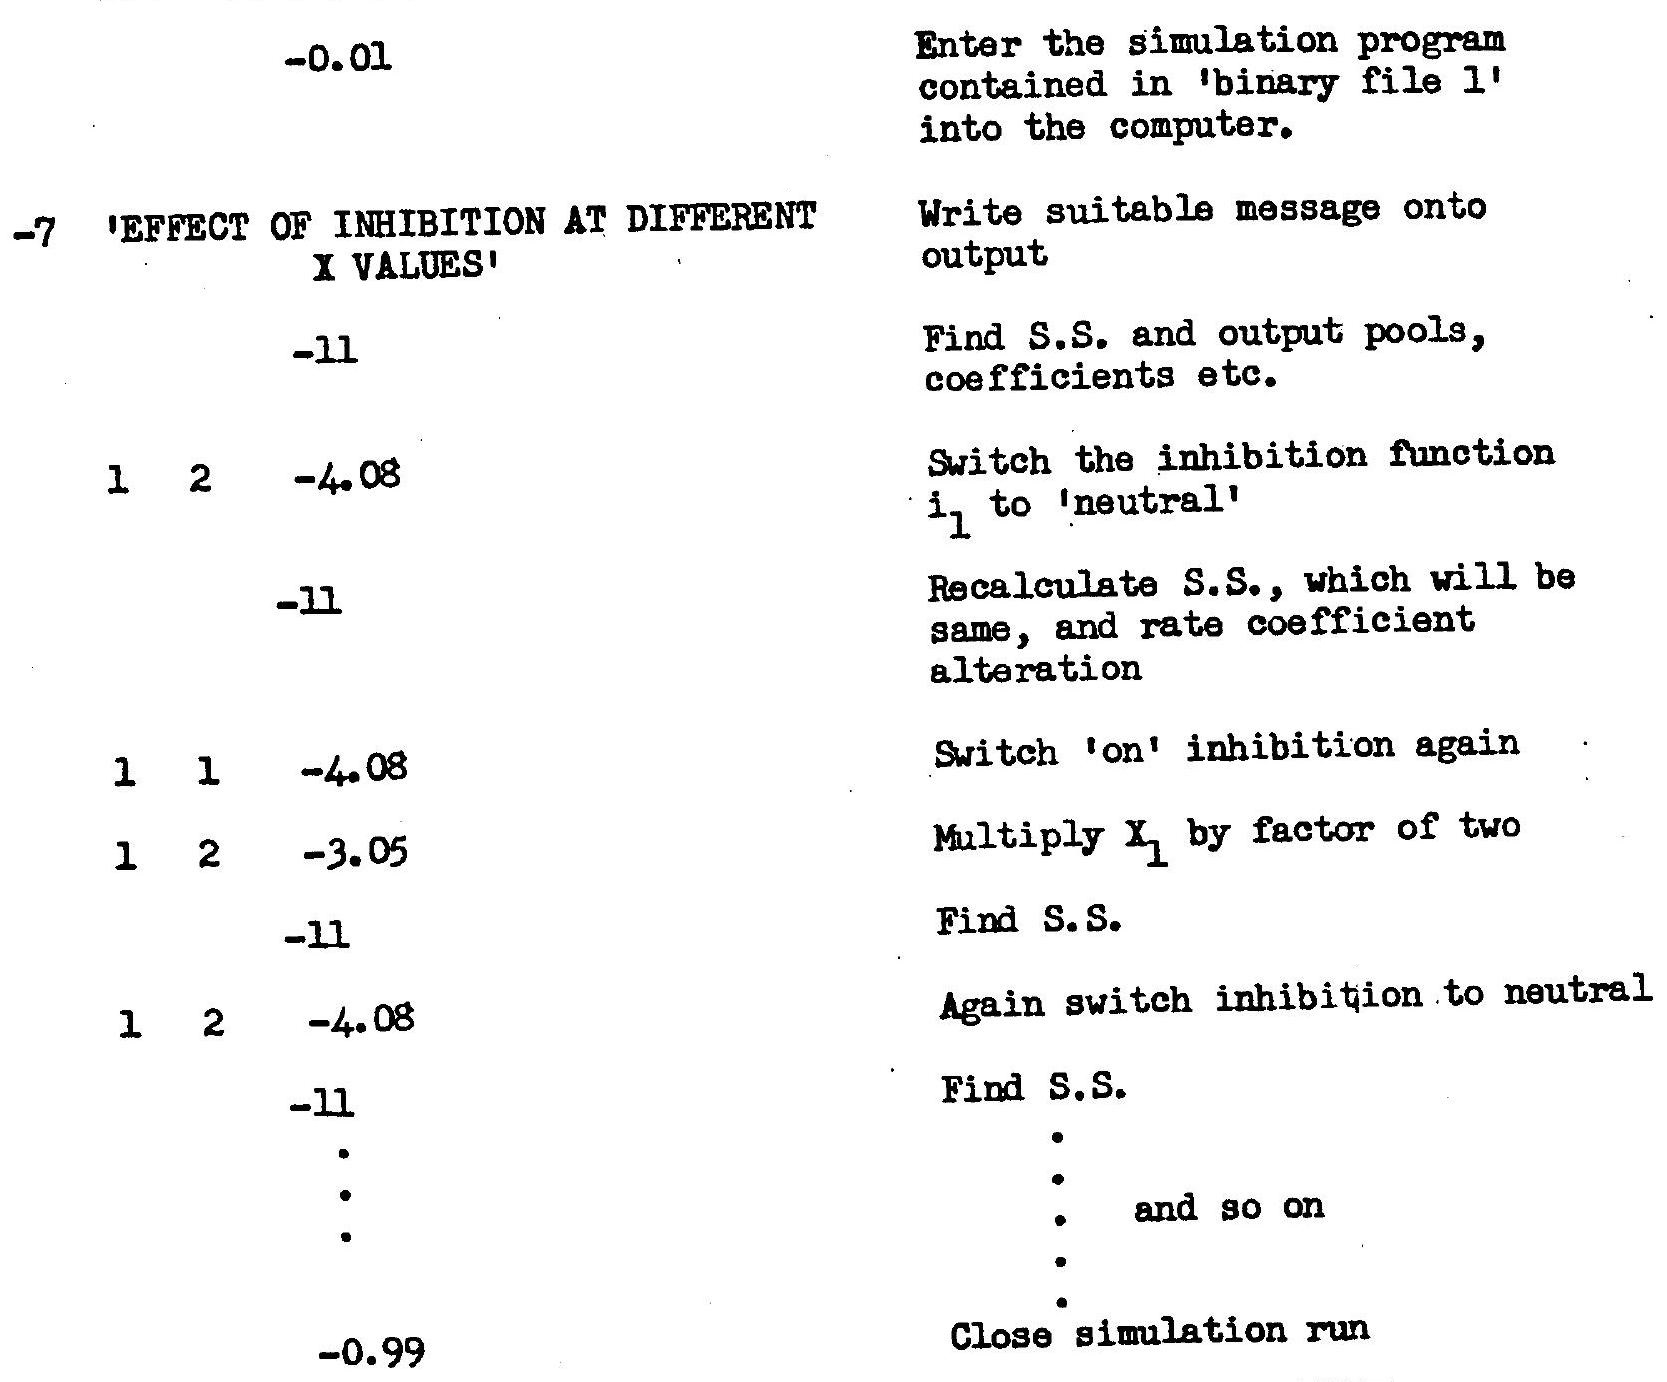
\includegraphics[max width=0.95\textwidth]{2023_01_30_a974a42f7b7381f3f940g-195}
\end{center}

The above experiment is intended to see what effect the presence of the inhibition $i_1$ has on the pattern of sensitivity coefficients for increasing levels of $X_1$

\section{The simulation program}

Here it seems useful to outline certain aspects of the program these being concerned broadly with the `numerical' techniques for locating the S.S. and the programming techniques for interpreting the simulation language. The overall program consists in declaring `arrays' for all the variable types involved, such as $\mathrm{E}, \mathrm{t}$ and $\mathrm{p}$, the size of these arrays being filled in by the precompiler at `load' time. Space is also declared for the matrix $\left[\frac{d \phi_{i}}{d S_{j}}\right]$ which is required. for the iteration procedure mentioned in $\mathrm{CH}$. I and also for

computation connected with the sensitivity coefficients, in addition a large `switch' is declared for use in selecting between the different commands. Following these declarations are a large number of routines each of which carries out a specified operation on the global `arrays' or is perhaps concerned with reading in and interpreting the simulation `language'.

\section{Working section}

The actual `working' part of the program is quite short and readable provided the routines which it uses have been given names which clearly indicate their function. It consists essentially of a multiple 'switch' which is selected on the basis of the lagt command. read in and is represented in the section below.

\begin{center}
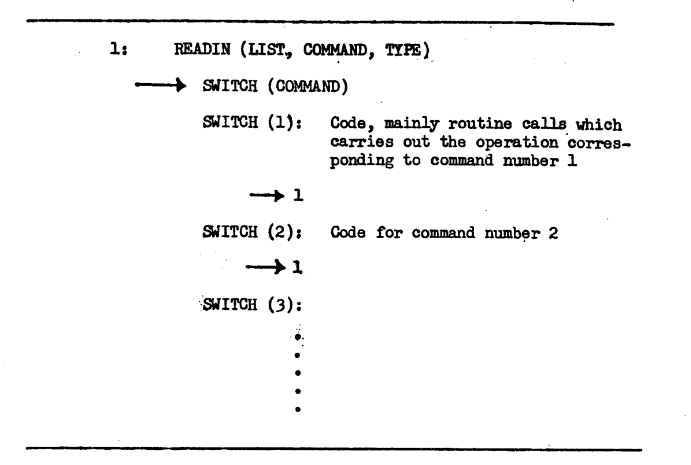
\includegraphics[max width=\textwidth]{figure4_4.png}
\end{center}

Let us consider the operation of the above assuming, for example, that the first line of the simulation language is {\tt \textquotesingle 1 10 4 5 -4.02\textquotesingle}

Starting at the 1st line, labelled (1:) the routine `READIN' fills the `array' LIST with the positive data $1,10,4,5$, sets the integer `COMMAND' to 4 and the integer `TYPE' to 2. On the next line the `SWITCH' instruction directed by the value of `COMMAND', will cause the program to jump to the line labelled SWITCH (4): which leads to a series of instructions designed to modify the specified quantities multiplicatively using the information contained in `LIST' and `TYPE'. When this operation is complete the instruction \kcmd{\hspace{40pt}1} is encountered and the program is ready to return to the routine `READIN' and obey the next command. The simulation program will thus read and obey any sequence of instructions until the input ceases. It can easily be seen, now, how the precompiler can `pick up' extra commands, if they are included with a network description at `load time', and attach them opposite the switch labels 20: and upwards which are left vacant in the standard simulator. Another point is that since each command expects to receive a certain data format it is a simple matter to check the contents of `LIST' and `TYPE' to see if they are legitimate. Such error detection facilities were extensively included in the KDF9 implementation and proved to be a valuable feature.

\section{Numerical aspects of locating the s.s. and estimating sensitivity coefficients}

One general way of getting into the neighbourhood of a steady state solution $\olsi{S}_{j}$ is to integrate the differential equations of motion (1.1), thus simulating the natural movement of the $S_{j} \cdot$ However, a criterion for when to stop, or indeed certainty as to whether one is in the region of a steady state at all, are not simple matters.

The criterion of closeness to the desired steady state is as follows; after every half hour of simulation (metabolic system time) the values of $(N - n)$ of the $F_{1}$ fluxes are accepted and the values of $F^{\prime}$ which the remaining $n$ must have in order to satisfy equation (1.1) with all $\dot{S}_{j}=0$ are calculated. In general these will be different from their existing values and

 $$=\sum \frac{F^{\prime}-F}{F} $$

is a measure of the distance of a constructed exact steady state, with slightly altered enzyme concentrations from the desired exact steady state with the prescribed enzyme concentrations. When the rate equations can be expressed in the form (1a) measures the sum of the fractional enzyme changes needed to move from the constructed to the prescribed steady state. Thus, if $0.001$. we can say that we have found a mathematically exact steady state such that no enzyme differs from its prescribed value by more than 1 part in 1000.

Simulation, which is costly, is only employed while 0.20. As soon as $0.20$ the matrix $\olsi{S}_j/\mathrm{E}_i$ is formed, by numerical approximation, for the constructed steady state and is used to estimate the $\olsi{S}_j$ obtaining at the correct enzyme values. This is repeated until is reduced to the required accuracy. This process, similar to Newton-Raphson iteration, converges rapidly for all systems so far tried and it is not necessary to recompute $\olsi{S}_j/E_i$ very frequently. The sensitivity coefficients $C_y^{x}$ can all be found from the matrix without appreciable further computation.

The time to recompute the $\olsi{S}_j/E_i$ matrix as we move about the parameter space is not great, compared with the time spent on simulation, for systems up to 30 enzymes. Also the necessary matrix inversion is numerically well-behaved provided that we already have a reasonable estimate for $\olsi{S}_j/E_i$, which will be the case if parameter movements are not too violent. Initial estimates of both $\olsi{S}_j$ and $\olsi{S}_j/E_i$ are more costly, being formed by simulation. They are computed only once and kept available should the current values be lost. Clearly the integration method employed can have a low accuracy and still suffice. At present 4th order Rutta-Merson is used because it is convenient and reliable. For "stiff" systems considerable improvement would result from the employment of a more suitable integration method.

